\usepackage[utf8]{inputenc, graphixc, caption, fullpage}

\section{Formulation}

We will be using Markov Models to find the probability of the events.
Markov models are graphs of events, that have weighted edges with the probability of their occurrence.
This graph is then converted into a matrix where the values in row $n$ column $i$ represent the odds of moving from $n$ to $i$.
This is a useful formulation because if you take the product of two of these matrices then it shows the odds of going from one state to another after 2 changes of state.
A proof, mostly to convince myself, is in Appendix I for the two by two case.

\subsection{Graphical Example}

\begin{figure}
  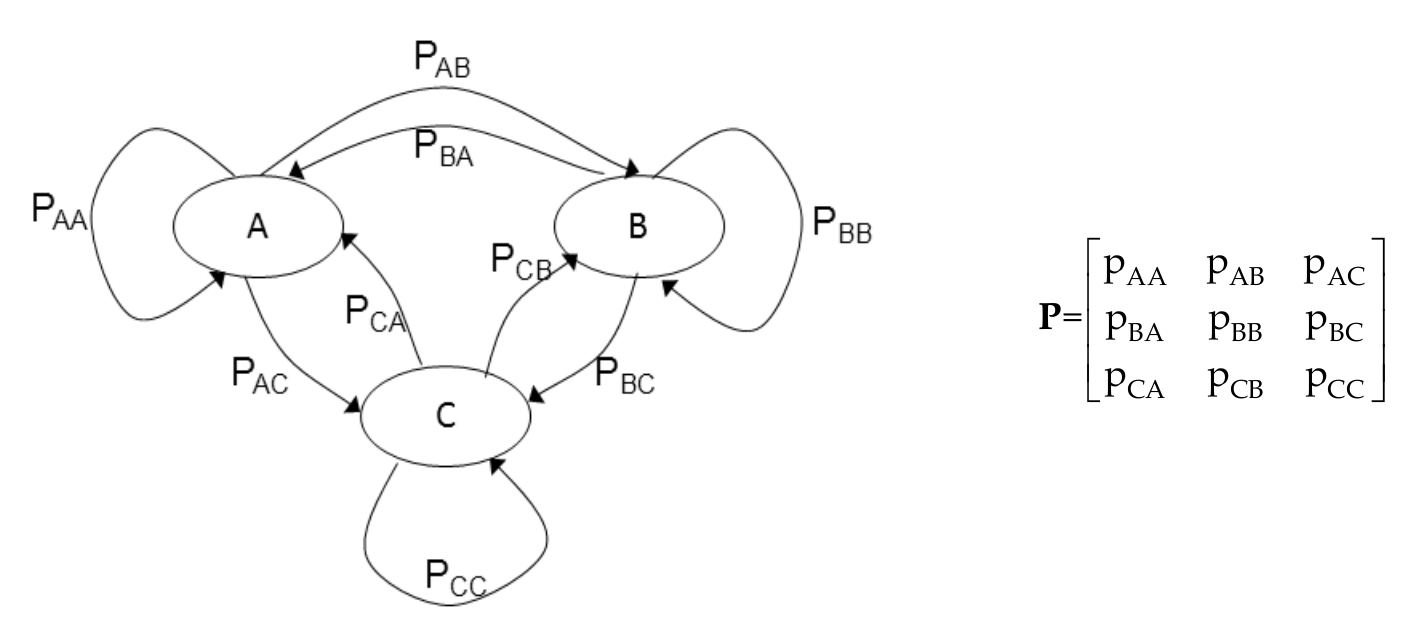
\includegraphics[width=\linewidth]{image11.jpeg}
  \label{Figure 1: Probability transition diagram for a 3-state Markov chain}
\end{figure}

Because we can use a matrix to represent a directed graph, we can use this matrix
to apply a weight to the edits and predict the outcome of events. Figure 1
shows an example of a graph and the corresponding matrix.\footnote{http://www.intechopen.com/books/matlab-a-fundamental-tool-for-scientific-computing-and-engineering-applications-volume-2/wireless-channel-model-with-markov-chains-using-matlab}

To find the odds of a transition, $P$ can be multiplied by the column vector
$\mathbf{x}=({P_A, P_B, P_C})^T$, where $P_X$ is the probability that the system
is in state $X$. So, $P\mathbf{x}$ results in the probability after one set
of changes, and $P(P\mathbf{x})$ results in the probability after two state
changes. This can be simplified to $P(P\mathbf{x} = (PP)\mathbf{x} = P^2\mathbf{x}$.
This can be further generalized to state that the probability after $n$ state
changes is: $P^n\mathbf{x}$. In the case of Yahtzee, we can use this to optimize
how we play so that we can consistently beat other players.
